\documentclass[a4paper]{article}

\def\npart {III}
\def\nterm {Michaelmas}
\def\nyear {2016}
\def\nlecturer {H. C. Johansson}
\def\ncourse {Local Fields}
\def\nlectures {MWF.10}

% Imports
\ifx \nextra \undefined
  \usepackage[pdftex,
    hidelinks,
    pdfauthor={Dexter Chua},
    pdfsubject={Cambridge Maths Notes: Part \npart\ - \ncourse},
    pdftitle={Part \npart\ - \ncourse},
  pdfkeywords={Cambridge Mathematics Maths Math \npart\ \nterm\ \nyear\ \ncourse}]{hyperref}
  \title{Part \npart\ - \ncourse}
\else
  \usepackage[pdftex,
    hidelinks,
    pdfauthor={Dexter Chua},
    pdfsubject={Cambridge Maths Notes: Part \npart\ - \ncourse\ (\nextra)},
    pdftitle={Part \npart\ - \ncourse\ (\nextra)},
  pdfkeywords={Cambridge Mathematics Maths Math \npart\ \nterm\ \nyear\ \ncourse\ \nextra}]{hyperref}

  \title{Part \npart\ - \ncourse \\ {\Large \nextra}}
\fi

\author{Lectured by \nlecturer \\\small Notes taken by Dexter Chua}
\date{\nterm\ \nyear}

\usepackage{alltt}
\usepackage{amsfonts}
\usepackage{amsmath}
\usepackage{amssymb}
\usepackage{amsthm}
\usepackage{booktabs}
\usepackage{caption}
\usepackage{enumitem}
\usepackage{fancyhdr}
\usepackage{graphicx}
\usepackage{mathtools}
\usepackage{microtype}
\usepackage{multirow}
\usepackage{pdflscape}
\usepackage{pgfplots}
\usepackage{siunitx}
\usepackage{tabularx}
\usepackage{tikz}
\usepackage{tkz-euclide}
\usepackage[normalem]{ulem}
\usepackage[all]{xy}

\pgfplotsset{compat=1.12}

\pagestyle{fancyplain}
\lhead{\emph{\nouppercase{\leftmark}}}
\ifx \nextra \undefined
  \rhead{
    \ifnum\thepage=1
    \else
      \npart\ \ncourse
    \fi}
\else
  \rhead{
    \ifnum\thepage=1
    \else
      \npart\ \ncourse\ (\nextra)
    \fi}
\fi
\usetikzlibrary{arrows}
\usetikzlibrary{decorations.markings}
\usetikzlibrary{decorations.pathmorphing}
\usetikzlibrary{positioning}
\usetikzlibrary{fadings}
\usetikzlibrary{intersections}
\usetikzlibrary{cd}

\newcommand*{\Cdot}{\raisebox{-0.25ex}{\scalebox{1.5}{$\cdot$}}}
\newcommand {\pd}[2][ ]{
  \ifx #1 { }
    \frac{\partial}{\partial #2}
  \else
    \frac{\partial^{#1}}{\partial #2^{#1}}
  \fi
}

% Theorems
\theoremstyle{definition}
\newtheorem*{aim}{Aim}
\newtheorem*{axiom}{Axiom}
\newtheorem*{claim}{Claim}
\newtheorem*{cor}{Corollary}
\newtheorem*{defi}{Definition}
\newtheorem*{eg}{Example}
\newtheorem*{fact}{Fact}
\newtheorem*{law}{Law}
\newtheorem*{lemma}{Lemma}
\newtheorem*{notation}{Notation}
\newtheorem*{prop}{Proposition}
\newtheorem*{thm}{Theorem}

\renewcommand{\labelitemi}{--}
\renewcommand{\labelitemii}{$\circ$}
\renewcommand{\labelenumi}{(\roman{*})}

\let\stdsection\section
\renewcommand\section{\newpage\stdsection}

% Strike through
\def\st{\bgroup \ULdepth=-.55ex \ULset}

% Maths symbols
\newcommand{\bra}{\langle}
\newcommand{\ket}{\rangle}

\newcommand{\N}{\mathbb{N}}
\newcommand{\Z}{\mathbb{Z}}
\newcommand{\Q}{\mathbb{Q}}
\renewcommand{\H}{\mathbb{H}}
\newcommand{\R}{\mathbb{R}}
\newcommand{\C}{\mathbb{C}}
\newcommand{\Prob}{\mathbb{P}}
\renewcommand{\P}{\mathbb{P}}
\newcommand{\E}{\mathbb{E}}
\newcommand{\F}{\mathbb{F}}
\newcommand{\cU}{\mathcal{U}}
\newcommand{\RP}{\mathbb{RP}}
\newcommand{\CP}{\mathbb{CP}}

\newcommand{\ph}{\,\cdot\,}

\DeclareMathOperator{\sech}{sech}
\DeclareMathOperator{\cosech}{cosech}
\DeclareMathOperator{\cosec}{cosec}

\DeclareMathOperator{\covol}{covol}
\DeclareMathOperator{\vol}{vol}

\let\Im\relax
\let\Re\relax
\DeclareMathOperator{\Im}{Im}
\DeclareMathOperator{\Re}{Re}
\DeclareMathOperator{\im}{im}
\DeclareMathOperator{\image}{image}
\DeclareMathOperator{\Ann}{Ann}

\DeclareMathOperator*{\res}{res}
\DeclareMathOperator{\Res}{Res}
\DeclareMathOperator{\Ind}{Ind}

\DeclareMathOperator{\tr}{tr}
\DeclareMathOperator{\diag}{diag}
\DeclareMathOperator{\rank}{rank}
\DeclareMathOperator{\card}{card}
\DeclareMathOperator{\spn}{span}
\DeclareMathOperator{\adj}{adj}

\DeclareMathOperator{\erf}{erf}
\DeclareMathOperator{\erfc}{erfc}

\DeclareMathOperator{\ord}{ord}
\DeclareMathOperator{\Sym}{Sym}

\DeclareMathOperator{\sgn}{sgn}
\DeclareMathOperator{\orb}{orb}
\DeclareMathOperator{\stab}{stab}
\DeclareMathOperator{\ccl}{ccl}

\DeclareMathOperator{\lcm}{lcm}
\DeclareMathOperator{\hcf}{hcf}

\DeclareMathOperator{\Int}{Int}
\DeclareMathOperator{\id}{id}

\DeclareMathOperator{\betaD}{beta}
\DeclareMathOperator{\gammaD}{gamma}
\DeclareMathOperator{\Poisson}{Poisson}
\DeclareMathOperator{\binomial}{binomial}
\DeclareMathOperator{\multinomial}{multinomial}
\DeclareMathOperator{\Bernoulli}{Bernoulli}
\DeclareMathOperator{\like}{like}

\DeclareMathOperator{\var}{var}
\DeclareMathOperator{\cov}{cov}
\DeclareMathOperator{\bias}{bias}
\DeclareMathOperator{\mse}{mse}
\DeclareMathOperator{\corr}{corr}

\DeclareMathOperator{\otp}{otp}
\DeclareMathOperator{\dom}{dom}

\DeclareMathOperator{\Root}{Root}
\DeclareMathOperator{\supp}{supp}
\DeclareMathOperator{\rel}{rel}
\DeclareMathOperator{\Hom}{Hom}
\DeclareMathOperator{\Aut}{Aut}
\DeclareMathOperator{\Gal}{Gal}
\DeclareMathOperator{\Mat}{Mat}
\DeclareMathOperator{\End}{End}
\DeclareMathOperator{\Char}{char}
\DeclareMathOperator{\ev}{ev}
\DeclareMathOperator{\St}{St}
\DeclareMathOperator{\Lk}{Lk}
\DeclareMathOperator{\disc}{disc}
\DeclareMathOperator{\Isom}{Isom}
\DeclareMathOperator{\length}{length}
\DeclareMathOperator{\energy}{energy}
\DeclareMathOperator{\area}{area}
\DeclareMathOperator{\Syl}{Syl}
\DeclareMathOperator{\cl}{cl}
\DeclareMathOperator{\fix}{fix}

\newcommand{\GL}{\mathrm{GL}}
\newcommand{\SL}{\mathrm{SL}}
\newcommand{\PGL}{\mathrm{PGL}}
\newcommand{\PSL}{\mathrm{PSL}}
\newcommand{\PSU}{\mathrm{PSU}}
\newcommand{\Or}{\mathrm{O}}
\newcommand{\SO}{\mathrm{SO}}
\newcommand{\U}{\mathrm{U}}
\newcommand{\SU}{\mathrm{SU}}

\renewcommand{\d}{\mathrm{d}}
\newcommand{\D}{\mathrm{D}}

\tikzset{->/.style = {decoration={markings,
                                  mark=at position 1 with {\arrow[scale=2]{latex'}}},
                      postaction={decorate}}}
\tikzset{<-/.style = {decoration={markings,
                                  mark=at position 0 with {\arrowreversed[scale=2]{latex'}}},
                      postaction={decorate}}}
\tikzset{<->/.style = {decoration={markings,
                                   mark=at position 0 with {\arrowreversed[scale=2]{latex'}},
                                   mark=at position 1 with {\arrow[scale=2]{latex'}}},
                       postaction={decorate}}}
\tikzset{->-/.style = {decoration={markings,
                                   mark=at position #1 with {\arrow[scale=2]{latex'}}},
                       postaction={decorate}}}
\tikzset{-<-/.style = {decoration={markings,
                                   mark=at position #1 with {\arrowreversed[scale=2]{latex'}}},
                       postaction={decorate}}}

\tikzset{circ/.style = {fill, circle, inner sep = 0, minimum size = 3}}
\tikzset{mstate/.style={circle, draw, blue, text=black, minimum width=0.7cm}}

\definecolor{mblue}{rgb}{0.2, 0.3, 0.8}
\definecolor{morange}{rgb}{1, 0.5, 0}
\definecolor{mgreen}{rgb}{0.1, 0.4, 0.2}
\definecolor{mred}{rgb}{0.5, 0, 0}

\def\drawcirculararc(#1,#2)(#3,#4)(#5,#6){%
    \pgfmathsetmacro\cA{(#1*#1+#2*#2-#3*#3-#4*#4)/2}%
    \pgfmathsetmacro\cB{(#1*#1+#2*#2-#5*#5-#6*#6)/2}%
    \pgfmathsetmacro\cy{(\cB*(#1-#3)-\cA*(#1-#5))/%
                        ((#2-#6)*(#1-#3)-(#2-#4)*(#1-#5))}%
    \pgfmathsetmacro\cx{(\cA-\cy*(#2-#4))/(#1-#3)}%
    \pgfmathsetmacro\cr{sqrt((#1-\cx)*(#1-\cx)+(#2-\cy)*(#2-\cy))}%
    \pgfmathsetmacro\cA{atan2(#2-\cy,#1-\cx)}%
    \pgfmathsetmacro\cB{atan2(#6-\cy,#5-\cx)}%
    \pgfmathparse{\cB<\cA}%
    \ifnum\pgfmathresult=1
        \pgfmathsetmacro\cB{\cB+360}%
    \fi
    \draw (#1,#2) arc (\cA:\cB:\cr);%
}
\newcommand\getCoord[3]{\newdimen{#1}\newdimen{#2}\pgfextractx{#1}{\pgfpointanchor{#3}{center}}\pgfextracty{#2}{\pgfpointanchor{#3}{center}}}

\def\Xint#1{\mathchoice
   {\XXint\displaystyle\textstyle{#1}}%
   {\XXint\textstyle\scriptstyle{#1}}%
   {\XXint\scriptstyle\scriptscriptstyle{#1}}%
   {\XXint\scriptscriptstyle\scriptscriptstyle{#1}}%
   \!\int}
\def\XXint#1#2#3{{\setbox0=\hbox{$#1{#2#3}{\int}$}
     \vcenter{\hbox{$#2#3$}}\kern-.5\wd0}}
\def\ddashint{\Xint=}
\def\dashint{\Xint-}


\begin{document}
\maketitle
{\small
\setlength{\parindent}{0em}
\setlength{\parskip}{1em}

The $p$-adic numbers $\Q_p$ (where $p$ is any prime) were invented by Hensel in the late 19th century, with a view to introduce function-theoretic methods into number theory. They are formed by completing $\Q$ with respect to the $p$-adic absolute value $|-|_p$ , defined for non-zero $x \in \Q$ by $|x|_p = p^{-n}$, where $x = p^n a/b$ with $a, b, n \in \Z$ and $a$ and $b$ are coprime to $p$. The $p$-adic absolute value allows one to study congruences modulo all powers of $p$ simultaneously, using analytic methods. The concept of a local field is an abstraction of the field $\Q_p$, and the theory involves an interesting blend of algebra and analysis. Local fields provide a natural tool to attack many number-theoretic problems, and they are ubiquitous in modern algebraic number theory and arithmetic geometry.

Topics likely to be covered include:
\begin{itemize}[label={}]
  \item The $p$-adic numbers. Local fields and their structure.
  \item Finite extensions, Galois theory and basic ramification theory.
  \item Polynomial equations; Hensel's Lemma, Newton polygons.
  \item Continuous functions on the $p$-adic integers, Mahler's Theorem.
  \item Local class field theory (time permitting).
\end{itemize}

\subsubsection*{Pre-requisites}
Basic algebra, including Galois theory, and basic concepts from point set topology and metric spaces. Some prior exposure to number fields might be useful, but is not essential.
}
\tableofcontents
\setcounter{section}{-1}
\section{Introduction}
What are local fields? Suppose we are interested in some basic number theoretic problem. Say we have a polynomial $f(x_1, \cdots, x_n) \in \Z[x_1, \cdots, x_n]$. We want to look for solutions $\mathbf{a} \in \Z^n$, or show that there are no solutions at all. We might try to view this polynomial as a real polynomial, look at its roots, and see if they are integers. In lucky cases, we might be able to show that there are no real solutions at all, and conclude that there cannot be any solutions at all.

On the other hand, we can try to look at it modulo some prime $p$. If there are no solutions mod $p$, then there cannot be any solution. But sometimes $p$ is not enough. We might want to look at it mod $p^2$, or $p^3$, or \ldots. One important application of local fields is that we can package all these information together. In this course, we are not going to study the number theoretic problems, but just look at the properties of the local fields for their own sake.

Throughout this course, all rings will be commutative with unity, unless otherwise specified.
\section{Basic theory}
We are going to start with some generalities.
\begin{defi}[Absolute value]\index{absolute value}
  Let $K$ be a field. An \emph{absolute value} on $K$ is a function $|\ph|: K \to \R_{\geq 0}$ such that
  \begin{enumerate}
    \item $|x| = 0$ iff $x = 0$;
    \item $|xy| = |x||y|$ for all $x, y \in K$;
    \item $|x + y| \leq |x| + |y|$.\index{triangle inequality}
  \end{enumerate}
\end{defi}

\begin{defi}[Valued field]\index{valued field}
  A \emph{valued field} is a field with an absolute value.
\end{defi}

\begin{eg}
  The rationals, reals and complex numbers with the usual absolute values are absolute values.
\end{eg}

\begin{eg}[Trivial absolute value]
  The \emph{trivial absolute value}\index{trivial absolute value} on a field $K$ is the absolute value given by
  \[
    |x| =
    \begin{cases}
      1 & x \not= 0\\
      0 & x = 0
    \end{cases}.
  \]
\end{eg}
From now on, we assume our absolute values are non-trivial.

There are some familiar basic properties of the absolute value such as
\begin{prop}
  $||x| - |y|| \leq |x - y|$. Here the outer absolute value on the left hand side is the usual absolute value of $\R$, while the others are the absolute values off the relevant field.
\end{prop}

An absolute value defines a metric $d(x, y) = |x - y|$ on $K$.

\begin{defi}[Equivalence of absolute values]\index{absolute values!equivalence}\index{equivalent absolute values}
  Let $K$ be a field, and let $|\ph|, |\ph|'$ be absolute values. We say they are \emph{equivalent} if they induce the same topology.
\end{defi}

\begin{ex}
  Using the same notation as above, show that the following are equivalent:
  \begin{enumerate}
    \item $|\ph|$ and $|\ph|'$ are equivalent
    \item $|x| < 1$ implies $|x|' < 1$ for all $x \in K$
    \item There is some $s \in \R_{> 0}$ such that $|x|^s = |x|'$ for all $x \in K$.
  \end{enumerate}
\end{ex}

\begin{ex}
  Let $K$ be a valued field. Then equivalent absolute values induce the same the \emph{completion} $\hat{K}$ of $K$, and $\hat{K}$ is a valued field with an absolute value extending $|\ph|$.
\end{ex}

\begin{defi}[Non-archimedean absolute value]\index{non-archimedean absolute value}\index{absolute value!non-archimedean}\index{archimedean absolute value}\index{absolute value!archimedean}
  An absolute value $|\ph|$ on a field $K$ is called \emph{non-archimedean} if $|x + y| \leq \max(|x|, |y|)$. This condition is called the \emph{strong triangle inequality}\index{strong triangle inequality}.

  An absolute value which isn't non-archimedean is called \emph{archimedean}.
\end{defi}
Metrics satisfying $d(x, z) \leq \max(d(x, y), d(y, z))$ are often known as \emph{ultrametrics}\index{ultrametric}.

\begin{eg}
  $\Q$, $\R$ and $\C$ under the usual absolute values are archimedean.
\end{eg}

However, in this course, we will only consider non-archimedean absolute values. Thus, from now on, unless otherwise mentioned, an absolute value is assumed to be non-archimedean. The metric is weird!

\begin{eg}
  Let $(K, |\ph|)$ be a non-archimedean valued field. let $x \in K$ and $r \in \R_{> 0}$. Let
  \[
    B(x, r) = \{y: |x - y| \leq r\}.
  \]
  We pick $z \in B(x, r)$, and suppose $y$ is such that $|y - z| \leq r$, ie. $y \in B(z, r)$. Then
  \[
    |x - y| = |(x - z) + (z - y)| \leq \max(|x - z|, |z - y|) \leq r.
  \]
  So $y \in B(x, r)$. So we conclude that $B(z, r) \subseteq B(x, r)$. By symmetry, we have $B(x, r) = B(z, r)$! Thus, closed balls do not have unique ``centers''. Every point can be viewed as the center.

  In particular, we have
  \[
    \{y: |y - z| < r\} \subseteq B(z, r) = B(x, r)
  \]
  for all $z \in B(x, r)$. So the closed ball $B(x, r)$ is open as well! (In the other direction, open balls are also closed!)
\end{eg}
\begin{prop}
  Let $K$ be a non-archimedean valued field, and $x, y \in K$. If $|x| > |y|$, then $|x + y| = |x|$.

  More generally, if $x = \sum_{c = 0}^\infty x_\ell$ and the non-zero $|x_i|$ are distinct, then $|x| = \max |x_i|$.
\end{prop}

\begin{proof}
  On the one hand, we have $|x + y| \leq \max\{|x|, |y|\}$. On the other hand, we have
  \[
    |x| = |(x + y) - y| \leq \max(|x + y|, |y|) = |x + y|.
  \]
  So we must have $|x| = |x + y|$.
\end{proof}

\begin{prop}
  Let $K$ be a valued field. Then
  \[
    \mathcal{O} = \{x: |x| \leq 1\}
  \]
  is an open subring of $K$, called the \emph{valuation ring of K}. Moreover, for each $r \in (0, 1]$, we have $\{x : |x| < r\}$ and $\{x: |x| \leq r\}$ are open ideals of $\mathcal{O}$. Moreover, $\mathcal{O}^\times = \{x : |x| = 1\}$.
\end{prop}

\begin{proof}
  We know that these sets are open by the previous example.

  To see $\mathcal{O}$ is a subring, we have $|1| = |-1| = 1$. So $1, -1 \in \mathcal{O}$. If $x, y \in \mathcal{O}$, then $|x + y| \leq \max(|x|, |y|) \leq 1$. So $x + y \in \mathcal{O}$. Also, $|xy| = |x||y| \leq 1 \cdot 1 = 1$. So $xy \in \mathcal{O}$.

  That the other sets are ideals of $\mathcal{O}$ is checked in the same way.

  To check the units, we have $x \in \mathcal{O}^\times \Leftrightarrow |x|, |x^{-1}| \leq 1 \Leftrightarrow |x| = |x|^{-1} = 1$.
\end{proof}

\begin{defi}[Valuation ring]\index{valuation ring}
   Let $K$ be a valued field. Then the \emph{valuation ring of K}\index{valuation ring} is the open subring
  \[
    \mathcal{O} = \{x: |x| \leq 1\}.
  \]
\end{defi}
We start to see how these non-archimedean fields have more interesting algebraic properties than our usual fields.

\begin{prop}
  Let $K$ be a valued field.
  \begin{enumerate}
    \item Let $(x_n)$ be a sequence in $K$. If $x_n - x_{n + 1} \to 0$, then $x_n$ is Cauchy.
  \end{enumerate}
  If we assume further that $K$ is complete, then
  \begin{enumerate}[resume]
    \item Let $(x_n)$ be a sequence in $K$. If $x_n - x_{n + 1} \to 0$, then a sequence $(x_n)$ in $K$ converges.
    \item Let $\sum_{n = 0}^\infty y_n$ be a series in $K$. If $y_n \to 0$, then $\sum_{n = 0}^\infty y_n$ converges.
  \end{enumerate}
\end{prop}
The converses to all these are of course also true, with the usual proofs.

\begin{proof}\leavevmode
  \begin{enumerate}
    \item Pick $\varepsilon > 0$ and $N$ such that $|x_n - x_{n + 1}| < \varepsilon$ for all $n \geq N$. Then given $m\geq n \geq N$, we have
      \begin{align*}
        |x_m - x_n| &= |x_m - x_{m - 1} + x_{m - 1} - x_{m - 2} + \cdots - x_n| \\
        &\leq \max(|x_m - x_{m - 1}|, \cdots, |x_{n + 1} - x_n|) \\
        &< \varepsilon.
      \end{align*}
      So the sequence is Cauchy.
    \item Follows from (1) and the definition of completeness.
    \item Follows from the definition of convergence of a series and (2).
  \end{enumerate}
\end{proof}

\begin{defi}[Integral element]\index{integral element}
  Let $R \subseteq S$ be rings and $s \in S$. We say $s$ is \emph{integral over $R$} if there is some monic $f \in R[x]$ such that $f(s) = 0$.
\end{defi}

\begin{eg}
  Any $r \in R$ is integral (take $f(x) = x - r$).
\end{eg}

\begin{eg}
  Take $\Z \subseteq \C$. Then $z \in \C$ is integral over $\Z$ if it is an \term{algebraic integer} (by definition of algebraic integer).
\end{eg}

\begin{defi}[Adjoint/Adjugate matrix]
  Let $A = (a_{ij})$ be an $n \times n$ matrix with coefficients in a ring $R$. The \term{adjugate matrix} or \term{adjoint matrix} $A^* = (a_{ij}^*)$ of $A$ is defined by
  \[
    a_{ij}^* = (-1)^{i + j} \det (A_{ij}),
  \]
  where $A_{ij}$ is an $(n-1)\times (n-1)$ matrix obtained from $A$ by deleting the $i$th column and the $j$th row.
\end{defi}

\begin{prop}
  For any $A$, we have $A^*A = AA* = \det(A) I$, where $I$ is the identity matrix.
\end{prop}

\begin{prop}
  Let $R \subseteq S$ be rings. Then $s_1, \cdots, s_n \in S$ are all integral iff $R[s_1, \cdots, s_n] \subseteq S$ is a finitely-generated $R$-module.
\end{prop}
Note that $R[s_1, \cdots, s_n]$ is by definition a finitely-generated $R$-algebra, but requiring it to be finitely-generated as a module is stronger.

\begin{proof}
  Note that we can construct $R[s_1, \cdots, s_n]$ by a sequence
  \[
    R \subseteq R[s_1] \subseteq R[s_1, s_2] \subseteq \cdots \subseteq R[s_1, \cdots, s_n] \subseteq S,
  \]
  and each $s_i$ is integral over $R[s_1, \cdots, s_{n - 1}]$. Since the finite extension of a finite extension is still finite, it suffices to prove it for the case $n = 1$, and we write $s$ for $s_1$.

  Suppose $f(x) \in R[[x]$ is monic such that $f(s) = 0$. If $g(x) \in R[x]$, then there is some $q, r \in R[x]$ such that $g(x) = f(x)q(x) + r(x)$ with $\deg r < \deg f$. Then $g(s) = r(s)$. So any polynomial expression in $s$ can be written as a polynomial expression with degree less than $\deg f$. So $R[s]$ is generated by $1, s, \cdots, s^{\deg f - 1}$.

  In the other direction, let $t_1, \cdots, t_d$ be $R$-module generators of $R[s_1, \cdots, s_n]$. Now let $b \in R[s_1, \cdots, s_n]$. Then there is some $a_{ij} \in R$ such that
  \[
    b t_i = \sum_{j = 1}^d a_{ij} t_j.
  \]
  In matrix form, this says
  \[
    (bI - A)t = 0.
  \]
  We now multiply by $(bI - A)^*$ to obtain
  \[
    \det(bI - A) t_j = 0
  \]
  for all $j$. Now we know $1 \in R$. So $1 = \sum c_j t_j$ for some $c_j \in R$. Then we have
  \[
    \det(bI - A) = \det(bI - A) \sum c_j t_j = \sum c_j (\det (bI - A) t_j) = 0.
  \]
  Since $\det(bI - A)$ is a monic polynomial in $b$, it follows that $b$ is integral. In particular, the generators $s_i$ are integral.
\end{proof}

\begin{cor}
  Let $R \subseteq S$ be rings. If $s_1, s_2 \in S$ are integral over $R$, then $s_1 + s_2$ and $s_1s_2$ are integral over $R$. In particular, the set $\tilde{R} \subseteq S$ of all elements in $S$ integral over $R$ is a ring, known as the integral closure of $R$ in $S$.
\end{cor}

\begin{proof}
  If $s_1, s_2$ are integral, then $R[s_1, s_2]$ is a finite extension over $R$. Since $s_1 + s_2$ and $s_1s_2$ are elements of $R[s_1, s_2]$, they are also integral over $R$.
\end{proof}

\begin{defi}[Integrally closed]
  Given a ring extension $R \subseteq S$, we say $R$ is \term{integrally closed} in $S$ if $\tilde{R} = R$.
\end{defi}

\begin{defi}[Topological ring]\index{topological ring}\index{ring topology}
  Let $R$ be a ring. A topology on $R$ is called a \emph{ring topology} if addition and multiplication are continuous maps $R \times R \to R$. A ring with a ring topology is a \emph{topological ring}.
\end{defi}

\begin{eg}
  $\R$ and $\C$ with the usual topologies and usual ring structures are topological rings.
\end{eg}

\begin{ex}
  Let $K$ be a valued field. Then $K$ is a topological ring. We can see this from the fact that the product topology on $K \times K$ is induced by the metric $d((x_0, y_0), (x_1, y_1)) = \max(|x_0 - x_1|, |y_0 - y_1|)$.
\end{ex}

\begin{defi}[$i$-adically open]\index{$I$-adically open}
  Let $R$ be a ring and $I \subseteq R$ an ideal. A subset $U \subseteq R$ is called \emph{$I$-adically open} if for all $x \in U$, there is some $n \geq 1$ such that $x + I^n \subseteq U$.
\end{defi}

\begin{prop}
  The set of all $I$-adically open sets form a topology on $R$, called the $I$-adic topology.
\end{prop}

\begin{proof}
  By definition, we have $\emptyset$ and $R$ are open, and arbitrary unions are clearly open. if $U, V$ are $I$-adically open, and $x \in U \cap V$, then there are $n, m$ such that $x + I^n \subseteq U$ and $x + I^m \subseteq V$. Then $x + I^{\max(m, n)} \subseteq U \cap V$.
\end{proof}

\begin{ex}
  Check that the $I$-adic topology is a ring topology.
\end{ex}

\begin{defi}[Inverse/projective limit]\index{inverse limit}\index{projective limit}
  Let $R_1, R_2,, \cdots$ be topological rings, with continuous homomorphisms $f_n: R_{n + 1} \to R_n$.
  \[
    \begin{tikzcd}
      R_1 & R_2 \ar[l, "f_1"] & R_3 \ar[l, "f_2"] & R_4 \ar[l, "f_3"] & \ar[l] \cdots
    \end{tikzcd}
  \]
  The \emph{inverse limit} or \emph{projective limit} of the $R_i$ is the ring
  \[
    \varprojlim R_n = \left\{(x_n) \in \prod_n R_n : f_n(x_{n + 1}) = x_n\right\},
  \]
  with coordinatewise addition and multiplication, together with the subspace topology coming from the product topology of $\prod R_n$. This topology is known as the \term{inverse limit topology}.
\end{defi}

\begin{prop}
  The inverse limit topology is a ring topology.
\end{prop}

\begin{proof}[Proof sketch]
  We can fit the addition and multiplication maps into diagrams
  \[
    \begin{tikzcd}
      \varprojlim R_n \times \varprojlim R_n \ar[r] & \varprojlim R_n\\
      \prod R_n \times \prod R_n \ar[u, hook] \ar[r] & \prod R_n \ar[u, hook]
    \end{tikzcd}
  \]
  By the definition of the subspace topology, it suffices to show that the corresponding maps on $\prod R_n$ are continuous. By the universal property of the product, it suffices to show that the projects $\prod R_n \times \prod R_n \to R_m$ is continuous for all $m$. But this map can alternatively be obtained by first projecting to $R_m$, then doing multiplication in $R_m$, and projection is continuous. So the result follows.
\end{proof}

\begin{defi}[$I$-adic completion]
  Let $R$ be a ring and $I$ be an ideal. The \term{$I$-adic completion} of $R$ is the topological ring
  \[
    \varprojlim R/I^n,
  \]
  where $R/I^n$ has the discrete topology, and $R/I^{n + 1} \to R/I^n$ is the obvious map. There is an evident map
  \begin{align*}
    \nu: R &\to \varprojlim R/I^n\\
    r &\mapsto (r \bmod I^n)_.
  \end{align*}
  This map is a continuonus ring homomorphism if $R$ is given the $I$-adic topology.
\end{defi}

\begin{defi}[$I$-adically complete]\index{$I$-adically complete}
  We say that $R$ is \emph{$I$-adically complete} if $\nu$ is a bijection.
\end{defi}

\begin{ex}
  If $\nu$ is a bijection, then $\nu$ is in fact a homeomorphism.
\end{ex}
If $I = xR$, when we often call the $I$-adic topology the \term{$x$-adic topology}.

\section{The $p$-adic numbers}
For the rest of this course, $p$ is going to be a prime number.

Let $x \in \Q$ be non-zero. Then by uniqueness of factorization, we can write $x$ uniquely as
\[
  x =p^n \frac{a}{b},
\]
where $a, b, n \in \Z$, $b > 0$ and $a, b, p$ are pairwise coprime.

\begin{defi}[$p$-adic absolute value]\index{$p$-adic absolute value}
  The \emph{$p$-adic absolute value} on $Q$ is the function $|\ph|_p: \Q \to \R_{\geq 0}$ given by
  \[
    |x|_p =
    \begin{cases}
      0 & x = 0\\
      p^{-n} & x = p^n \frac{a}{b}\text{ as above}
    \end{cases}.
  \]
\end{defi}

\begin{prop}
  The $p$-adic absolute value is an absolute value.
\end{prop}

\begin{proof}
  It is clear that $|x|_p = 0$ iff $x = 0$.

  Suppose we have
  \[
    x = p^n \frac{a}{b},\quad y = p^m \frac{c}{d}.
  \]
  We wlog $m \geq n$. Then we have
  \[
    |xy|_p = \left|p^{n + m}\frac{ac}{bd}\right| = p^{-m-n}|x|_p |y|_p.
  \]
  So this is multiplicative. Finally, we have
  \[
    |x + y|_p = \left|p^n \frac{ab + p^{m - n}cb}{bd}\right| \leq p^{-n} = \max(|x|_p, |y|_p).
  \]
  Note that we must have $bd$ coprime to $p$, but $ab + p^{m - n}cb$ need not be. However, any extra powers of $p$ could only decrease the absolute value, hence the above result.
\end{proof}

Note that if $x \in \Z$ is an integer, then $|x|_p = p^{-n}$ iff $p^n \mid\mid x$ (we say $p^n \mid\mid x$ if $p^n \mid x$ and $p^{n + 1} \nmid x$).

\begin{defi}[$p$-adic numbers]\index{$p$-adic numbers}
  The \emph{$p$-adic numbers} $\Q_p$ is the completion of $\Q$ with respect to $|\ph|_p$.
\end{defi}

\begin{defi}[$p$-adic integeres]\index{$p$-adic integers}
  The valuation ring
  \[
    \Z_p = \{x \in \Q_p: |x|_p \leq 1\}
  \]
  is the \emph{$p$-adic integers}.
\end{defi}

\begin{prop}
  $\Z_p$ is the closure of $\Z$ inside $\Q_p$.
\end{prop}

\begin{proof}
  If $x \in \Z$ is non-zero, then $x = p^na$ with $n \geq 0$. So $|x|_p \leq 1$. So $\Z \subseteq \Z_p$.

  We now want to show that $\Z$ is dense in $\Z_p$. We know the set
  \[
    \Z_{(p)} = \{x \in \Q: |x|_p \leq 1\}
  \]
  is dense inside $\Z_p$, essentially by definition. So it suffices to show that $\Z$ is dense in $\Z_{(p)}$. We let $x \in \Z_{(p)} \setminus\{0\}$, say
  \[
    x = p^n \frac{a}{b},\quad n \geq 0.
  \]
  It suffices to find $x_i \in \Z$ such that $x_i \to \frac{1}{b}$. Then we have $p^n ax_i \to x$.

  Since $(b, p) = 1$, we can find $x_i, y_i \in \Z$ such that $b x_i + p^i y_i = 1$ for all $i \geq 1$. So
  \[
    \left|x_i - \frac{1}{b}\right|_p = \left|\frac{1}{b}\right|_p |bx_i - 1|_p = |p^i y_i|_p \leq p^{-i} \to 0.
  \]
  So done.
\end{proof}

\begin{prop}
  The non-zero ideals of $\Z_p$ are $p^n \Z_p$ for $n \geq 0$. Moreover,
  \[
    \frac{\Z}{p^n \Z} \cong \frac{\Z_p}{p^n \Z_p}.
  \]
\end{prop}

\begin{proof}
  Let $0 \not= I \subseteq \Z_p$ be an ideal, and pick $x \in I$ such that $|x|_p$ is maximal. This supremum exists and is attained because the possible values of the absolute values are discrete and bounded above. If $y \in I$, then by maximality, we have $|y|_p \leq |x|_p$. So we have $|yx^{-1}|_p \leq 1$. So $yx^{-1} \in \Z_p$, and this implies that $y = (yx^{-1})x \in x\Z_p$. So $I \subseteq x\Z_p$, and we obviously have $x\Z_p \subseteq I$. So we have $I = x\Z_p$.

  Now if $x = p^n \frac{a}{b}$, then since $\frac{a}{b}$ is invertible in $\Z_p$, we have $x\Z_p = p^n \Z_p$. So $I = p^n \Z_p$.

  To show the second part, consider the map
  \[
    f_n: \Z \to \frac{\Z_p}{p^n \Z_p}
  \]
  given by the inclusion map followed by quotienting. Now $p^n \Z_p = \{x : |x|_p \leq p^{-n}$. So we have
  \[
    \ker f_n = \{x \in \Z: |x|_p \leq p^{-n}\} = p^n \Z.
  \]
  Now since $\Z$ is dense in $\Z_p$, we know $f_n$ is surjective (let $x \in \Z_p$. Then by density, there is an integer in the $p^{-n}$-ball of $x$, and this belongs to the same $p^n \Z_p$ equivalence class as $x$). So $f_n$ induces an isomorphism $\Z/p^n Z \cong \Z_p/p^n \Z_p$.
\end{proof}

\begin{cor}
  $\Z_p$ is a PID with a unique prime element $p$ (up to units).
\end{cor}
This is pretty much the point of the $p$-adic numbers --- there are a lot of primes in $\Z$, and by passing on to $\Z_p$, we are left with just one of them.

\begin{prop}
  The topology on $\Z$ induced by $|\ph|_p$ is the $p$-adic topology (ie. the $p\Z$-adic topology).
\end{prop}

\begin{proof}
  Let $U \subseteq \Z$. By definition, $U$ is open wrt $|\ph|_p$ iff for all $x \in U$, there is an $n\in \N$ such that
  \[
    \{y \in \Z: |y - x|_p \leq p^{-n}\} \subseteq U.
  \]
  On the other hand, $U$ is open in the $p$-adic topology iff for all $x \in U$, there is some $n \geq 0$ such that $x + p^n \Z \subseteq U$. But we have
  \[
    \{y \in \Z: |y - x|_p \leq p^{-n}\} = x + p^n \Z.
  \]
  So done.
\end{proof}

\begin{prop}
  $\Z_p$ is $p$-adically complete and is (isomorphic to) the $p$-adic completion of $\Z$.
\end{prop}

\begin{proof}
  The second part follows from the first as follows: we have the maps
  \[
    \begin{tikzcd}
      \Z_p \ar[r, "\nu"] & \varprojlim \Z_p/(p^n \Z_p) & \lim \Z/(p^n\Z) \ar[l, "(f_n)_n"]
    \end{tikzcd}
  \]
  We know the map induced by $(f_n)_n$ is an isomorphism. So we just have to show that $\nu$ is an isomorphism

  To prove the first part, we have $x \in \ker \nu$ iff $x \in p^n \Z_p$ for all $n$ iff $|x|_p \leq p^{-n}$ for all $n$ iff $|x|_p = 0$ iff $x = 0$. So the map is injective.

  To show surjectivity, we let
  \[
    z_n \in \varprojlim \Z_p/p^n \Z_p.
  \]
  We define $a_i \in \{0, 1, \cdots, p - 1\}$ recursively such that
  \[
    x_n = \sum_{i = 0}^{n - 1} a_i p^i
  \]
  is the unique representative of $z_n$ in the set of integers $\{0, 1, \cdots, p^n - 1\}$. Then
  \[
    x = \sum_{i = 0}^\infty a_i p^i
  \]
  exists in $\Z_p$ and maps to $x \equiv x_n \equiv z_n \pmod{p^n}$ for all $n \geq 0$. So $\nu(x) = (z_n)$. So the map is surjective. So $\nu$ is bijective.
\end{proof}

\begin{cor}
  Every $a \in \Z_p$ has a unique expansion
  \[
    a = \sum_{i = 0}^\infty a_i p^i.
  \]
  with $a_i \in \{0, \cdots, p - 1\}$.

  More generally, for any $a \in \Q^\times$, there is a unique expansion
  \[
    a = \sum_{i = n}^\infty a_i p^i
  \]
  for $a_i \in \{0, \cdots, p - 1\}$, $a_n \not= 0$ and
  \[
    n = - \log_p |a|_p \in \Z.
  \]
\end{cor}

\begin{proof}
  The second part follows from the first part by multiplying $a$ by $p^{-n}$.
\end{proof}

\begin{eg}
  We have
  \[
    \frac{1}{1 - p} = 1 + p + p^2 + p^3 + \cdots.
  \]
\end{eg}

\section{Valued fields}
We return to the discussion of general valued fields.
\begin{defi}[Valuation]
  Let $K$ be a field. A \term{valuation} on $K$ is a function $v: K \to \R \cup \{\infty\}$ such that
  \begin{enumerate}
    \item $v(x) = 0$ iff $x = 0$
    \item $v(xy) = v(x) + v(y)$
    \item $v(x + y) \geq \min\{v(x), v(y)\}$.
  \end{enumerate}
\end{defi}
Here we use the conventions that $r + \infty = \infty$ and $r \leq \infty$ for all $r \in \infty$.

In some sense, this definition is sort-of pointless, since if $v$ is a valuation, then the function
\[
  |x| = c^{-v(x)}
\]
for any $c > 1$ is a (non-archimedean) absolute value. Conversely, if $|\ph|$ is a valuation, then
\[
  v(x) = - \log_c |x|
\]
is a valuation.

Despite this, sometimes people prefer to talk about the valuation rather than the absolute value, and often this is more natural.

\begin{eg}
  For $x \in \Q_p$, we define
  \[
    v_p(x) = -\log_p |x|_p.
  \]
  This is a valuation, and if $x \in \Z_p$, then $v_p(x) = n$ iff $p^n \mid\mid x$.
\end{eg}

\begin{eg}
  Let $K$ be a field, and define
  \[
    k((T)) = \left\{\sum_{i = n}^\infty a_i T^i: a_i \in k, n \in \Z\right\}.
  \]
  This is the field of \term{formal Laurent series} over $k$. We define
  \[
    v\left(\sum a_i T^i\right) = \min\{i: a_i \not= 0\}.
  \]
  Then $v$ is a valuation of $k((T))$.
\end{eg}

Recall that for a valued field $K$, the \term{valuation ring}\index{$\mathcal{O}_K$} is given by
\[
  \mathcal{O} = \mathcal{O}_K = \{x \in k; |x|\leq 1\}.
\]
Since this is a subring of a field, and the absolute value is multiplicative, we notice that the units in $\mathcal{O}$ are exactly the elements of absolute value $1$. The remaining elements form an ideal (since the field is non-archimedean), and thus we have a \term{maximal ideal}
\[
  \mathfrak{m} = \mathfrak{m}_K = \{x \in K: |x| < 1\}
\]
The quotient
\[
  k = k_K = \mathcal{O}_K/\mathfrak{m}
\]
is known as the \term{residue field}.

\begin{eg}
  Let $K = \Q_p$. Then $\mathcal{O} = \Z_p$, and $\mathfrak{m} = p\Z_p$. So
  \[
    k = \mathcal{O}/\mathfrak{m} = \Z_p/p\Z_p \cong \Z/p\Z.
  \]
\end{eg}

\begin{defi}[Primitive polynomial]\index{primitive polynomial}
  If $K$ is a valued field and $F(x) = a_0 + a_1 x + \cdots + a_n x^n \in K[x]$ is a polynomial, we say that $F$ is \emph{primitive} if
  \[
    \max_i |a_i| = 1.
  \]
  In particular, we have $F \in \mathcal{O}[x]$.
\end{defi}
The point of a primitive polynomial is that such a polynomial is naturally, and non-trivially, an element of $k[x]$. Moreover, focusing on such polynomials is not that much of a restriction, since any polynomial is a constant multiple of a primitive polynomial.

\begin{thm}[Hensel's lemma]\index{Hensel's lemma}
  Let $K$ be a complete valued field, and let $F \in K[x]$ be primitive. Put $f = F\bmod \mathfrak{m} \in k[x]$. If there is a factorization
  \[
    f(x) = g(x) h(x)
  \]
  with $(g, h) = 1$, then there is a factorization
  \[
    F(x) = G(x) H(x)
  \]
  in $\mathcal{O}[x]$ with
  \[
    g = G,\quad h = H\mod m,
  \]
  with $\deg g = \deg G$.
\end{thm}
Note that requiring $\deg g = \deg G$ is the best we can hope for --- we cannot guarantee $\deg h = \deg H$, since we need not have $\deg f = \deg F$.

This is one of the most important results in the course. Unfortunately, the proof is not terribly enlightening.

\begin{proof}
  Put $d = \deg F$ and $m = \deg g$. Then we have $\deg h \leq d - m$.

  We pick lifts $G_0, H_0 \in \mathcal{O}[x]$ of $g, h$ with $\deg G_0 = \deg g$, and $\deg H_0 \leq d - m$. Then we have
  \[
    F = G_0 H_0 \mod \mathfrak{m}.
  \]
  Our strategy is to add some correction terms to $G_0$ and $H_0$ so that the corresponding equation holds mod $\mathfrak{m}^2$, then lift to a result mod $\mathfrak{m}^3$ etc, \ldots and hopefully eventually get something in the limit.

  However, this doesn't really work, since there is no guarantee that the limit converges! The trick is to pick and element $\pi \in \mathfrak{m}$, and then work modulo $\pi^k$. This is not hard, since we notice that
  \[
    \pi \mathcal{O} = \{x \in \mathcal{O}: |x| \leq |\pi|\}.
  \]
  Since our equations only have finitely many coefficients, we can always replace $\bmod \mathfrak{m}$ with $\bmod \pi$ for large enough $\pi$.

  If we do this, then the correction terms we add in each iteration will be bounded by $|\pi|^k$, and thus tends to $0$. Now recall that a series converges iff the moduli of the terms tend to $0$! So we are done if this works.

  Before we begin, we use the given condition $(g, h) = 1$ to obtain some $A, B \in \mathcal{O}[x]$ such that
  \[
    AG_0 + B H_0 \equiv 1 \mod \mathfrak{m}.
  \]
  Then we know that
  \[
    F - G_0 H_0 \equiv AG_0 + BH_0 - 1 \equiv 0 \mod \mathfrak{m}.
  \]
  Thus, since the polynomials involved have finitely many coefficients, we can pick pick a $\pi \in \mathfrak{m}$ with large enough modulus such that
  \[
    F - G_0 H_0 \equiv AG_0 + BH_0 - 1 \equiv 0 \mod \pi.
  \]
  The idea is to find successive approximations
  \begin{align*}
    G_{n - 1} &= G_0 + \pi P_1 + \cdots + \pi^{n - 1} P_{n - 1},\\
    H_{n - 1} &= H_0 + \pi Q_1 + \cdots + \pi^{n - 1} Q_{n - 1}.
  \end{align*}
  that satisfy
  \[
    F \equiv G_{n - 1}H_{n - 1}\mod \pi^n.
  \]
  We then set
  \begin{align*}
    G &= G_0 + \pi P_1 + \pi^2 P_2 + \cdots,\\
    H &= H_0 + \pi Q_1 + \pi^2 Q_2 + \cdots.
  \end{align*}
  We then have $G \equiv G_i \mod \pi^{i + 1}$, and similarly for $H$. So we have
  \[
    F \equiv GH \mod \pi^n
  \]
  for all $n$. As $|\pi^n| \to 0$ as $n \to \infty$, we must have $F = GH$.

  We proceed by induction. Assume we already have $G_{n - 1}, H_{n - 1}$. We need to find $P_n, Q_n$ such that
  \begin{align*}
    G_n &= G_{n - 1} + \pi^n P_n\\
    H_n &= H_{n - 1} - \pi^n Q_n
  \end{align*}
  satisfy
  \[
    F - G_n H_n = 0\mod \pi^{n + 1}.
  \]
  Expanding $G_n$ and $H_n$ out, we get
  \[
    F - G_{n - 1}H_{n - 1} \equiv \pi^n (G_{m - 1} Q_n + H_{n - 1} P_n) \mod \pi^{n + 1}.
  \]
  We rearrange and divide by $\pi^n$ to obtain
  \[
    G_{n - 1} Q_n + H_{n - 1} P_n \equiv \frac{1}{\pi^n}(F - G_{n - 1}H_{n - 1}) \mod \pi.
  \]
  However, note that $G_{n - 1} = G_0 \mod \pi$ (and similarly for $H$), so we have
  \[
    G_0 Q_n + H_0 P_n \equiv \frac{1}{\pi^n}(F - G_{n - 1}H_{n - 1}) \mod \pi.
  \]
  We write
  \[
    E_n = \frac{1}{\pi^n}(F - G_{n - 1}H_{n - 1}).
  \]
  Now recall that there are $A, B$ such that
  \[
    AG_0 + B H_0 \equiv 1\mod \pi.
  \]
  Multiplying by $E_n$ thus gives
  \[
    E_n \equiv AG_0 E_n + B H_0 E_n\mod \pi.
  \]
  We might be tempted to set $Q_n$ and $P_n$ to be just $AE_n$ and $BE_n$ respectively, but we must control the degree of $P_n$ appropriately. Its degree must be less than $\deg g = \deg G_0$.

  Fortunately, the division algorithm comes to the rescue. Recall that $G_0$ is the lift of $g$ of the same degree, and thus its leading coefficient must be an element of $\mathcal{O} \setminus \mathfrak{m}$, ie. a unit. So we can perform the division algorithm to write
  \[
    B F_n = Q G_0 + P_n.
  \]
  with $\deg P_n < \deg G_0$. This gives the desired $P_n$. Then we have
  \[
    G_0 (A E_n + H_0 Q) + H_0 P_n \equiv E_n \mod \pi.
  \]
  Finally, let $Q_n = A E_n + H_0 Q$, where we drop all coefficients divisible by $\pi$. Then since $\deg E_n, \deg H_0 P_n \leq \deg F = m$, we must have $\deg Q_n \leq m - \deg G_0 = m - d$. So this has the desired degree as well. So done.
\end{proof}

\begin{cor}
  Let $F(x) = a_0 + a_1 x + \cdots + a_n x^n \in K[x]$ where $K$ is complete and $a_0, a_n \not= 0$. if $F$ is irreducible, then
  \[
    |a_\ell| \leq \max(|a_0|, |a_n|)
  \]
  for all $\ell$.
\end{cor}

\begin{proof}
  By scaling, we can wlog $F$ is primitive. Let $r$ be minimal such that $|a_r| = 1$. Then we have
  \[
    F(x) \equiv x^r (a_r + a_{r + 1}x + \cdots + a_n x^{n - r})\mod \mathfrak{m}.
  \]
  We want to prove that $\max(|a_0|, |a_n|) = 1$. If not, then $o < r < n$, and thus congruence lifts to a non-trivial factorization of $F$ by Hensel's lemma.
\end{proof}

\begin{cor}[of Hensel's lemma]
  Let $F \in \mathcal{O}[x]$ be monic, and $K$ complete. If $F \mod \mathfrak{m}$ has a simple root $\bar{\alpha} \in k$, then $F$ has a (unique) simple root $\alpha \in \mathcal{O}$ lifting $\bar{\alpha}$.
\end{cor}

\begin{eg}
  Consider $x^{p - 1} - 1 \in \Z_p[x]$. We know $x^{p - 1}$ splits into distinct linear factors over $\F_p[x]$. So all roots lift to $\Z_p$. So $x^{p - 1} - 1$ splits completely in $\Z_p$. So $\Z_p$ contains all $p$ roots of unity.
\end{eg}

\begin{thm}
  Let $K$ be a complete valued field, and let $L/K$ be a finite extension. Then the absolute value on $K$ has a unique extension to an absolute value on $L$, given by
  \[
    |\alpha|_L = \sqrt[n]{|N_{L/K}(\alpha)|},
  \]
  where $n = [L:K]$ and $N_{L/K}$ is the field norm. Moreover, $L$ is complete with respect to this absolute value.
\end{thm}

\begin{cor}
  Let $K$ be complete and $M/K$ be an algebraic extension of $K$. Then $|\ph|$ extends uniquely to an absolute value on $M$.
\end{cor}
This is since any algebraic extension is the union of finite extensions, and uniqueness means we can patch the absolute values together.

\begin{cor}
  Let $K$ be a complete valued field and $L/K$ a finite extension. if $\sigma \in \Aut(L/K)$, then $|\sigma(\alpha)|_L = |\alpha|_L$.
\end{cor}

\begin{proof}
  We check that $\alpha \mapsto |\sigma(\alpha)|_L$ is also an absolute value on $L$ extending the absolute value on $K$. So the result follows from uniqueness.
\end{proof}

Before we can prove the theorem, we need some preliminaries.
\begin{defi}[Norm on vector space]\index{norm on vector space}
  Let $K$ be a valued field and $V$ a vector space over $K$. A \emph{norm} on $V$ is a function $\norm{\ph}: V \to \R_{\geq 0}$ such that
  \begin{enumerate}
    \item $\norm{x} = 0$ iff $x = 0$.
    \item $\norm{\lambda} = |\lambda|\norm{x}$ for all $\lambda \in K$ and $x \in V$.
    \item $\norm{x + y} \leq \max \{\norm{x}, \norm{y}\}$.
  \end{enumerate}
\end{defi}

\begin{defi}[Equivalence of norms]\index{equivalence of norm}\index{norm!equivalent}
  Let $\norm{\ph}$ and $\norm{\ph}'$ be norms on $V$. Then two norms are equivalent if they induce the same otpology on $V$, ie. there are $C, D > 0$ such that
  \[
    C\norm{x} \leq \norm{x}'\leq D\norm{x}
  \]
  for all $x \in V$.
\end{defi}

\begin{prop}
  Let $K$ be a complete valued field, and $V$ a finite-dimensional $K$-vector space. Let $x_1, \cdots, x_n$ be a basis of $V$. Then if
  \[
    x = \sum a_i x_i,
  \]
  then
  \[
    \norm{x}_{\mathrm{max}} = \max_i |a_i|
  \]
  defines a norm on $V$, and moreover $V$ is complete with respect to $\norm{\ph}_{\mathrm{max}}$. Moreover, any other norm $\norm{\ph}$ on $V$ is equivalent to $\norm{\ph}_{\mathrm{max}}$. In particular, $V$ is complete with respect to any norm.
\end{prop}

\begin{proof}
  The proof that $\norm{\ph}_{\mathrm{max}}$ is indeed a norm and complete is left as an exercise for the reader.

  For the remaining part, let $\norm{\ph}$ be a norm. We need to find $C, D > 0$ such that
  \[
    C\norm{x}_{\mathrm{max}} \leq \norm{x} \leq D \norm{x}_{\mathrm{max}}.
  \]
  We set $D = \max_i(\norm{x})$. Then we have
  \[
    \norm{x} = \norm{\sum a_i x_i} \leq \max\left(\abs{a_i}\norm{x_i}\right) \leq (\max\abs{a_i}) D = \norm{x}_{\mathrm{max}}D.
  \]
  We find $C$ by induction on $n$. If $n = 1$, then $\norm{x} = \norm{a_1 x_1} = \abs{a_1} \norm{x} = \norm{x}_{\mathrm{max}}\norm{x_1}$. So $C = \norm{x_1}$ works.

  For $n \geq 2$, we let
  \begin{align*}
    V_i &= Kx_1 \oplus \cdots \oplus Kx_{i - 1} \oplus Kx_{i + 1} \oplus\cdots\oplus K x_n \\
    &= \spn\{x_1, \cdots, x_{i - 1}, x_{i + 1}, \cdots, x_n\}.
  \end{align*}
  By the induction hypothesis, each $V_i$ is complete with respect to (the restriction of) $\norm{\ph}$. So in particular $V_i$ is closed in $V$. So we know that the union
  \[
    \bigcup_{i = 1}^n x_i + V_i
  \]
  is also closed. By construction, this does not contain $0$. So there is some $C > 0$ such that if $x \in \bigcup_{i = 1}^n x_i + V_i$, then $\norm{x} \geq C$. We claim that
  \[
    C\norm{x}_{\mathrm{max}} \leq \|x\|.
  \]
  Indeed, take $x = \sum a_i x_i \in V$. Let $r$ be suh that
  \[
    |a_r| = \max_i (\abs{x_i}) = \norm{x}_{\mathrm{max}}.
  \]
  Then
  \begin{align*}
    \norm{x}_{\mathrm{max}}^{-1}\norm{x} &= \norm{a_r^{-1}x} \\
    &= \norm{\frac{a_1}{a_r}x_1 + \cdots + \frac{a_{r - 1}}{a_r} x_{r - 1} + x_r + \frac{a_{r + 1}}{a_r} x_{r + 1} + \cdots + \frac{a_n}{a_r}x_n}\\
    &\geq C,
  \end{align*}
  since the last vector is an element of $x_r + V_r$.
\end{proof}

\begin{lemma}
  Let $K$ be a valued field. Then the the valuation ring $\mathcal{O}_K$ is integrally closed in $K$.
\end{lemma}

\begin{proof}
  Let $x \in K$ and $|x| > 1$. Suppose we have $a_{n - 1}, \cdots, a_0 \in \mathcal{O}_k$. Then we have
  \[
    |x^n| > |a_0 + a_1x + \cdots + a_{n - 1} x^{n - 1}|.
  \]
  So we know
  \[
    x^n + a_{n - 1}x^{n - 1} + \cdots + a_1 x + a_0
  \]
  has non-zero norm, and in particular is non-zero. So $x$ is not integral over $\mathcal{O}_K$. So $\mathcal{O}_K$ is integrally closed.
\end{proof}

Finally, we get to prove our theorem.
\begin{thm}
  Let $K$ be a complete valued field, and let $L/K$ be a finite extension. Then the absolute value on $K$ has a unique extension to an absolute value on $L$, given by
  \[
    \abs{\alpha}_L = \sqrt[n]{\abs{N_{L/K}(\alpha)}},
  \]
  where $n = [L:K]$ and $N_{L/K}$ is the field norm. Moreover, $L$ is complete with respect to this absolute value.
\end{thm}

\begin{proof}
  For uniqueness and completeness, if $\abs{\ph}_L$ is an absolute value on $L$, then it is in particular a $K$-norm on $L$ as a finite-dimensional vector space. So we know $L$ is complete with respect to $\abs{\ph}_L$.

  If $\abs{\ph}_L'$ is another absolute value extending $\abs{\ph}$, then we know $\abs{\ph}_L$ and $\abs{\ph}_L'$ is equivalent in the sense of inducing the same topology. But then from one of the early exercises, when \emph{field} norms are equivalent, then we can find some $s > 0 $ such that $\abs{\ph}_L^s = \abs{\ph}_L'$. But the two norms agree on $K$, and they are non-trivial. So we must have $s = 1$. So the norms are equal.

  To show existence, we have to prove that
  \[
    \abs{\alpha}_L = \sqrt[n]{\abs{N_{L/K}(\alpha)}}
  \]
  is a norm.
  \begin{enumerate}
    \item If $\abs{\alpha}_L = 0$, then $N_{L/K}(\alpha) = 0$. This is true iff $\alpha = 0$.
    \item The multiplicativity of $\abs{\alpha}$ and follows from the multiplicativity of $N_{L/K}$, $\abs{\ph}$ and $\sqrt[n]{\ph}$.
  \end{enumerate}
  To show the strong triangle inequality, it suffices to show (cf. exercise 11 on example sheet 1) that $|\alpha|_L \leq 1$ implies $|\alpha + 1|_L \leq 1$.

  We know that
  \[
    \{\alpha \in L: \abs{\alpha}_L \leq 1\} = \{\alpha \in L: N_{L/K}(\alpha) \in \mathcal{O}_K\}.
  \]
  The claim is that this is equal to the integral closure of $\mathcal{O}_K$ in $L$. This implies what we want, since the integral closure is closed under addition (and $1$ is in the integral closure).

  Let $\abs{\alpha}_L \leq 1$. We wlog $\alpha \not= 0$, since that case is trivial. Let
  \[
    f(x) = a_0 + a_1x + \cdots + a_{n - 1}x^{n - 1} + x^n\in K[x]
  \]
  be the minimal polynomial of $\alpha$ over $K$. By the corollary of Hensel's lemma, for each $i$, we have
  \[
    |a_i| \leq \max(|a_0|, 1)
  \]
  By general properties of the field norm, there is some $m \in \Z_{\geq 1}$ such that $N_{L/K}(\alpha) = \pm a_0^m$. So we have
  \[
    |a_i| \leq \max\left(\abs{N_{L/K}(\alpha)^{1/m}}, 1\right) = 1.
  \]
  So $f \in \mathcal{O}_K[x]$. So $\alpha$ is integral over $\mathcal{O}_K$.

  On the other hand, suppose $\alpha$ is integral over $\mathcal{O}_K$. Let $\bar{K}/K$ be an algebraic closure of $K$. Note that
  \[
    N_{L/K}(\alpha) = \left(\prod_{\sigma: L \hookrightarrow \bar{K}} \sigma(\alpha)\right)^d,
  \]
  for some $d \in \Z_{\geq 1}$, and each $\sigma(\alpha)$ is integral over $\mathcal{O}_K$, since $\alpha$ is (apply $\sigma$ to the minimal polynomial). This implies that $N_{L/K}(\alpha)$ is integral over $\mathcal{O}_K$ (and lies in $K$). So $N_{L/K}(\alpha) \in \mathcal{O}_K$ since $\mathcal{O}_K$ is integrally closed in $K$.
\end{proof}

\begin{cor}[of the proof]
  Let $K$ be a complete valued field, and $L/K$ a finite extension. We equip $L$ with $|\ph|_L$ extending $|\ph|$ on $K$. Then $\mathcal{O}_L$ is the integral closure of $\mathcal{O}_K$ in $L$.
\end{cor}

\subsection{Newton polygons}
Newton polygons are some visual devices that tell us about roots of polynomials. It is very annoying to write down a formal definition, so we first look at some examples. We will work with valuations rather than the absolute value.

\begin{eg}
  Consider the valued field $(\Q_p, v_p)$, and the polynomial
  \[
    t^4 + p^2 t^4 - p^3 t^2 + pt + p^3.
  \]
  We then plot the coefficients for each power of $t$, and then draw a ``convex polygon'' so that all points lie on or above it:
  \begin{center}
    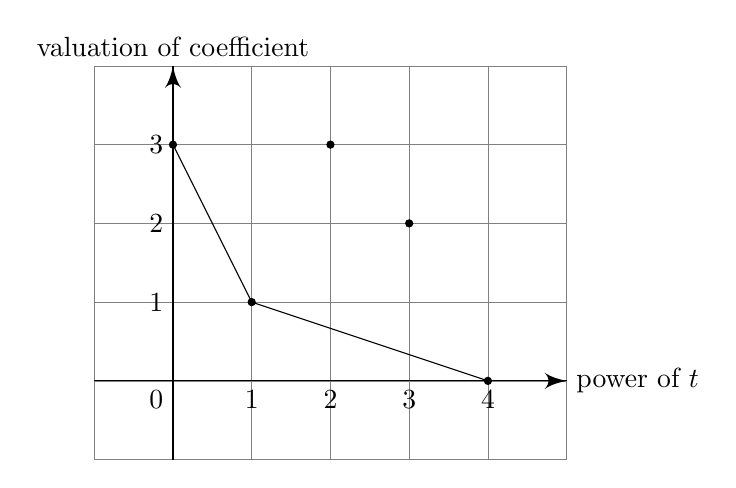
\begin{tikzpicture}
      \draw [step=1,gray, very thin] (-1, 4) grid (5, -1);

      \draw [->] (-1, 0) -- (5, 0) node [right] {power of $t$};
      \draw [->] (0, -1) -- (0, 4) node [above] {valuation of coefficient};

      \node [circ] at (0, 3) {};
      \node [circ] at (1, 1) {};
      \node [circ] at (2, 3) {};
      \node [circ] at (3, 2) {};
      \node [circ] at (4, 0) {};

      \draw (0, 3) -- (1, 1) -- (4, 0);

      \foreach \x in {1,2,3,4} {
        \node at (\x, 0) [below] {$\x$};
      }
      \node at (0, 0) [anchor = north east] {$0$};
      \foreach \y in {1,2,3} {
        \node at (0, \y) [left] {$\y$};
      }
    \end{tikzpicture}
  \end{center}
\end{eg}

\begin{eg}
  Consider $(\Q_2, v_2)$ with the polynomial
  \[
    4t^4 + 5t^3 + \frac{7}{2}t + \frac{9}{2}.
  \]
  Here there is no $t^2$ term, so we simply don't draw anything.
  \begin{center}
    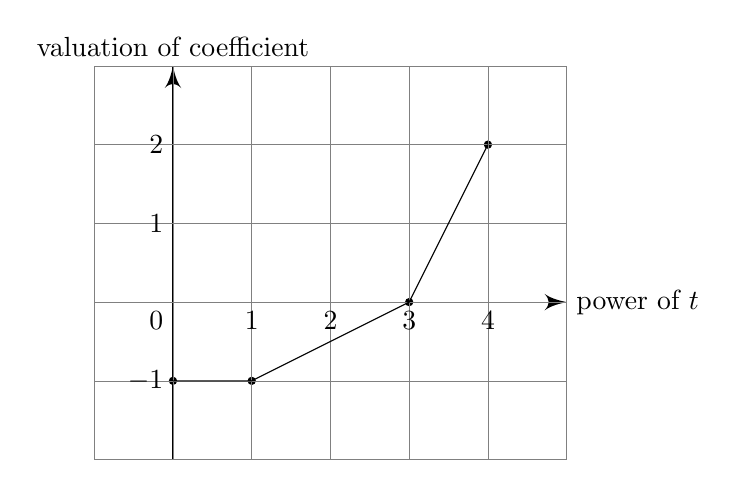
\begin{tikzpicture}
      \draw [->] (-1, 0) -- (5, 0) node [right] {power of $t$};
      \draw [->] (0, -2) -- (0, 3) node [above] {valuation of coefficient};

      \node [circ] at (0, -1) {};
      \node [circ] at (1, -1) {};
      \node [circ] at (3, 0) {};
      \node [circ] at (4, 2) {};

      \draw [step=1,gray, very thin] (-1, 3) grid (5, -2);
      \draw (0, -1) -- (1, -1) -- (3, 0) -- (4, 2);

      \foreach \x in {1,2,3,4} {
        \node at (\x, 0) [below] {$\x$};
      }
      \node at (0, 0) [anchor = north east] {$0$};
      \foreach \y in {-1,1,2} {
        \node at (0, \y) [left] {$\y$};
      }

    \end{tikzpicture}
  \end{center}
\end{eg}

We now go to come up with a formal definition.

\begin{defi}[Lower convex set]\index{lower convex set}
  We say a set $S \subseteq \R^2$ is \emph{lower convex} if
  \begin{enumerate}
    \item Whenever $(x, y) \in S$, then $(x, z) \in S$ for all $z \in \geq y$.
    \item $S$ is convex.
  \end{enumerate}
\end{defi}
\begin{defi}[Lower convex hull]
  Given any set of points $T \subseteq \R^2$, there is a minimal lower convex set $S \supseteq T$ (by the intersection of all lower convex sets containing $T$ -- this is a non-empty definition because $\R^2$ satisfies the property). This is known as the \term{lower convex hull} of the points.
\end{defi}

\begin{eg}
  The lower convex hull of the points $(0, 3), (1, 1), (2, 3), (3, 2), (4, 0)$ is given by the region denoted below:
   \begin{center}
    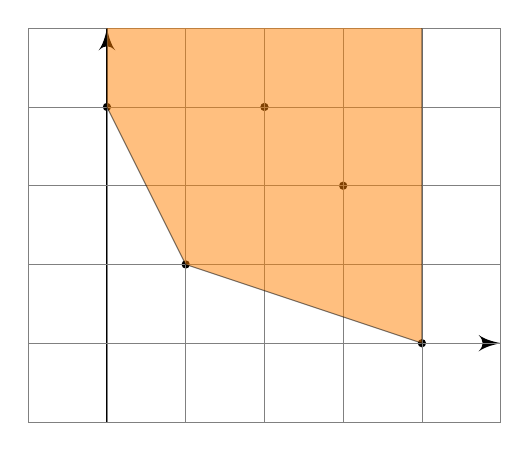
\begin{tikzpicture}
      \draw [->] (-1, 0) -- (5, 0);
      \draw [->] (0, -1) -- (0, 4);

      \node [circ] at (0, 3) {};
      \node [circ] at (1, 1) {};
      \node [circ] at (2, 3) {};
      \node [circ] at (3, 2) {};
      \node [circ] at (4, 0) {};

      \draw [step=1,gray, very thin] (-1, 4) grid (5, -1);
      \draw [fill=morange, opacity=0.5] (0, 4) -- (0, 3) -- (1, 1) -- (4, 0) -- (4, 4);
    \end{tikzpicture}
  \end{center}
\end{eg}

\begin{defi}[Newton polygon]\index{Newton polygon}
  Let $f(x) = a_0 + a_1 x + \cdots + a_n x^n \in K[x]$, where $(K, v)$ is a valued field. Then the \emph{Newton polygon} of $f$ is the lower convex hull of $\{(i, v(a_i)): i = 0, \cdots, n, a_i \not= 0\}$.
\end{defi}
This is the formal definition, so in our first example, the Newton polygon really should be the shaded area shown above, but most of the time, we only care about the lower line.

\begin{defi}[Break points]\index{break points}
  Given a polynomial, the points $(i, v(a_i))$ lying on the boundary of the Newton polygon are known as the \emph{break points}.
\end{defi}

\begin{defi}[Line segment]\index{line segment}
  Given a polynomial, the line segment between two adjacent break points is a \term{line segment}.
\end{defi}

\begin{defi}[Multiplicity/length]\index{multiplicity}\index{length}
  The \emph{length} or \emph{multiplicity} of a line segment is th e horizontal length.
\end{defi}

\begin{defi}[Slope]\index{slope}
  The \emph{slope} of a line segment is its slope.
\end{defi}

\begin{eg}
  Consider again $(\Q_2, v_2)$ with the polynomial
  \[
    4t^4 + 5t^3 + \frac{7}{2}t + \frac{9}{2}.
  \]
  \begin{center}
    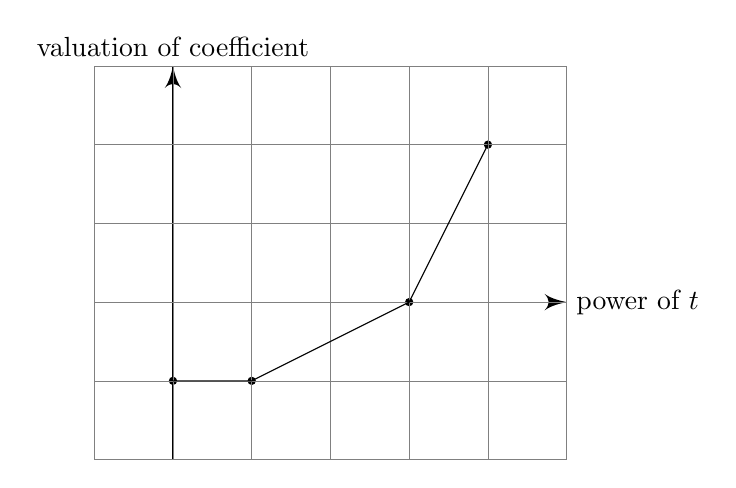
\begin{tikzpicture}
      \draw [->] (-1, 0) -- (5, 0) node [right] {power of $t$};
      \draw [->] (0, -2) -- (0, 3) node [above] {valuation of coefficient};

      \node [circ] at (0, -1) {};
      \node [circ] at (1, -1) {};
      \node [circ] at (3, 0) {};
      \node [circ] at (4, 2) {};

      \draw [step=1,gray, very thin] (-1, 3) grid (5, -2);
      \draw (0, -1) -- (1, -1) -- (3, 0) -- (4, 2);
    \end{tikzpicture}
  \end{center}
  The middle segment has length $2$ and slope $1/2$.
\end{eg}
\begin{eg}
  In the following Newton polygon:
  \begin{center}
    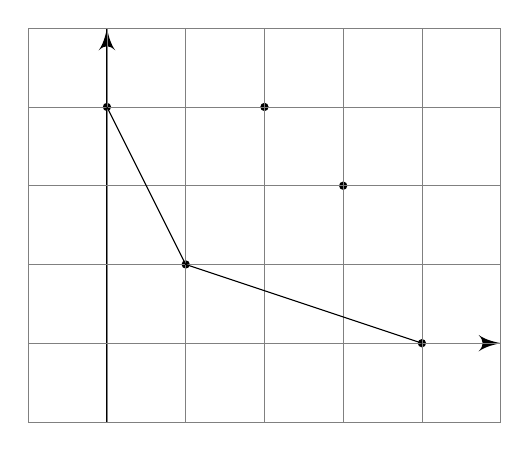
\begin{tikzpicture}
      \draw [->] (-1, 0) -- (5, 0);
      \draw [->] (0, -1) -- (0, 4);

      \node [circ] at (0, 3) {};
      \node [circ] at (1, 1) {};
      \node [circ] at (2, 3) {};
      \node [circ] at (3, 2) {};
      \node [circ] at (4, 0) {};

      \draw [step=1,gray, very thin] (-1, 4) grid (5, -1);
      \draw (0, 3) -- (1, 1) -- (4, 0);
    \end{tikzpicture}
  \end{center}
  The second line segment has length $3$ and slope $-\frac{1}{3}$.
\end{eg}

It turns out the Newton polygon tells us something about the roots of the polynomial.
\begin{thm}
  Let $K$ be complete valued field, and $v$ the valuation on $K$. We let
  \[
    f(x) = a_0 + a_1 x + \cdots + a_n x^n \in K[x].
  \]
  Let $L$ be the splitting field of $f$ over $K$, equipped with the unique extension $w$ of $v$.

  If $(r, v(a_r)) \to (s, v(a_s))$ is a line segment of the Newton polygon of $f$ with slope $-m \in \R$, then $f$ has precisely $s - r$ roots of valuation $m$.
\end{thm}
Note that by lower convexity, there can be at most one line segment for each slope. So this theorem makes sense.

\begin{proof}
  Dividing by $a_n$ only shifts the polygon vertically, so we may wlog $a_n = 1$. We number the roots of $f$ such that
  \begin{align*}
    w(\alpha_1) &= \cdots = w(\alpha_{s_1}) = w_1\\
    w(\alpha_{s_1 + 1} &= \cdots = w(\alpha_{s_2} = w_2\\
    &\vdots\\
    w(\alpha_{s_t}) &= \cdots = w(\alpha_n) = w_{t + 1},
  \end{align*}
  where we have
  \[
    w_1 < w_2 < \cdots < w_{t + 1}.
  \]
  Then we know
  \begin{align*}
    v(a_n) &= v(1) = 0\\
    v(a_{n - 1}) &= w\left(\sum \alpha_i\right) \geq \min_i w(\alpha_i) = w_1\\
    v(a_{n - 2}) &= w\left(\sum \alpha_i\alpha_j\right) \geq \min_{i \not= j} w(\alpha_i \alpha_j) = 2 m_1\\
    &\vdots\\
    v(a_{n - s_1} &= w\left(\sum_{i_1\not=\ldots \not=i_{s_1}} \alpha_{i_1 \ldots \alpha_{i_{s_1}}}\right) = \min w(\alpha_{i_1}\cdots\alpha_{i_{s_1}}) = s_1 m_1.
  \end{align*}
  It is important that in the last one, we have equality, not an inequality, because there is one term in the sum whose valuation is less than all the others.

  We can then continue to get
  \[
    v(\alpha_{n - s_1 - 1}) \geq \min w(\alpha_{i_1} \cdots \alpha_{i_{s_1 + 1}}) = s_1 m_1 + m_2,
  \]
  until we reach
  \[
    v(\alpha_{n - s_1 - s_2}) = s_1 m_1 + (s_2 - s_1) m_2.
  \]
  We keep going on.

  We draw the Newton polygon.
  \begin{center}
    \begin{tikzpicture}
      \draw [->] (-1, 0) -- (8, 0);
      \draw [->] (0, -2) -- (0, 2);

      \node [circ] at (7, 0) {};
      \node [above] at (7, 0) {$(n, 0)$};

      \node [circ] at (5, -1) {};
      \node [right] at (5, -1) {$(n - s_1, s_1 m_1)$};

      \node [circ] at (3, -1.5) {};
      \node [below] at (3, -1.5) {$(n - s_1 - s_2, s_1 m_1 + (s_2 - s_1) m_1)$};

      \node at (2, -1.5) {$\cdots$};

      \draw (7, 0) -- (5, -1) -- (3, -1.5);
    \end{tikzpicture}
  \end{center}
  We don't know where exactly the other points are, but the inequalities imply that the $(i, v(a_i))$ are above the lines drawn. So this is the Newton polygon.

  Counting from the right, the first line segment has length $n - (n - s_1) = s_1$ and slope
  \[
    \frac{0 - s_1 m_1}{n - (n - s_1)} = -m_1.
  \]
  In general, the $k$th segment has length $(n - s_{k - 1}) - (n - s_k) = s_k - s_{k - 1}$, and slope
  \begin{align*}
    &\frac{\left(s_1 m_1 + \sum_{i = 1}^{k - 2} (s_{i + 1} - s_i) m_{i + 1}\right) - \left(s_1 m_1 + \sum_{i = 1}^{k - 1} (s_{i + 1} - s_i) m_{i + 1}\right)}{s_k - s_{k - 1}} \\
    ={}& \frac{-(s_k - s_{k - 1})m_k}{s_k - s_{k - 1}} = - m_k.
  \end{align*}
  and the others follow similarly.
\end{proof}

\begin{cor}
  If $f$ is irreducible, then the Newton polygon has a single line segment.
\end{cor}

\begin{proof}
  We need to show that all roots have the same valuation. Let $\alpha, \varsigma$ be in the splitting field $L$. Then there is some $\sigma \in \Aut(L/K)$ such that $\sigma(\alpha) = \beta$. Then $w(\alpha) = w(\sigma(\alpha)) = \beta$. So done.
\end{proof}

\section{Discretely valued fields}
\begin{defi}[Discretely valued field]\index{discretely valued field}\index{valued field!discretely}\index{DVF}
  Let $K$ be a valued field with valuation $v$. We say $K$ is a \emph{discretely valued field} (DVF) if $v(k^\times) \subseteq \R$ is a discrete subgroup of $\R$, ie. $v(k^\times)$ is infinite cyclic.
\end{defi}

\begin{defi}[Local field]\index{local field}
  A complete discretely valued field with a finite residue field is called a \emph{local field}.
\end{defi}

\begin{defi}[Uniformizer]\index{uniformizer}
  Let $K$ be a discrete valued field. We say $\pi \in K$ is \emph{uniformizer} if $v(\pi) > 0$ and $v(\pi)$ generates $v(k^\times)$ (iff $v(\pi)$ has minimal positive valuation).
\end{defi}

\begin{eg}
  $\Q$ and $\Q_p$ with $v_p$ are both discretely valued fields, and $\Q_p$ is a local field. $p$ is a uniformizer.
\end{eg}

\begin{eg}
  The Laurent series field $k((T))$ with valuation
  \[
    v\left(\sum a_n T^n\right) = \inf\{n: a_n \not= 0\}
  \]
  is a discrete valued field, and is a local field if and only if $k$ is finite field. We have
  \[
    \mathcal{O}_{k((T))} = k[[T]] = \left\{\sum_{n = 0}^\infty a_n T^n: a_n \in k\right\}.
  \]
  Here $T$ is a uniformizer.
\end{eg}

These discretely valued field are pretty much like the $p$-adic numbers.
\begin{prop}
  Let $K$ be a discretely valued field with uniformizer $\pi$. Let $S \subseteq \mathcal{O}_K$ be a set of coset representatives of $\mathcal{O}_k/\mathfrak{m}_k = k_K$ containing $0$. Then
  \begin{enumerate}
    \item The non-zero ideals of $\mathcal{O}_K$ are $\pi^n \mathcal{O}_K$ for $n \geq 0$.
    \item The ring $\mathcal{O}_K$ is a PID with unique prime $\pi$ (up to units), and $\mathfrak{m}_K = \pi\mathcal{O}_K$.
    \item The topology on $\mathcal{O}_K$ induced by the absolute value is the $\pi$-adic topology.
    \item If $K$ is complete, then $\mathcal{O}_K$ is $\pi$-adically complete
    \item if $K$ is complete, then any $x \in K$ can be written uniquely as
      \[
        x = \sum_{n \gg -\infty}^\infty a_n \pi^n,
      \]
      where $a_n \in S$, and
      \[
        |x| = |\pi|^{-\inf\{n: a_n \not= 0\}}.
      \]
    \item The completion $\hat{K}$ is also discretely valued and $\pi$ is a uniformizer, and moreover the natural map
      \[
        \begin{tikzcd}
          \frac{\mathcal{O}_k}{\pi^n \mathcal{O}_k} \ar[r, "\sim"] & \frac{\mathcal{O}_{\hat{K}}}{\pi^n \mathcal{O}_{\hat{K}}}
        \end{tikzcd}
      \]
      is an isomorphism.
  \end{enumerate}
\end{prop}

\begin{proof}
  The same as for $\Q_p$ and $\Z_p$, with $\pi$ instead of $p$.
\end{proof}

\begin{prop}
  Let $K$ be a discretely valued field. Then $K$ is a local field iff $\mathcal{O}_K$ is compact.
\end{prop}

\begin{proof}
  If $\mathcal{O}_K$ is compact, then $\pi^{-n}\mathcal{O}_K$ is compact for all $n \geq 0$ (where $\pi$ is the uniformizer), and in particular complete. So
  \[
    K = \bigcup_{n \geq 0}^\infty \pi^{-n} \mathcal{O}_K
  \]
  is complete, as this is an increasing union, and Cauchy sequences are bounded. Also, we know the quotient map $\mathcal{O}_K \to k_K$ is continuous when $k_K$ is given the discrete topology, by definition of the $\pi$-adic topology. So $k_K$ is compact and discrete, hence finite.

  In the other direction, if $K$ is local, then we know $\mathcal{O}_K/\pi^n \mathcal{O}_K$ is finite for all $n \geq 0$ (by induction and finiteness of $k_K$). We let $(x_i)$ be a sequence in $\mathcal{O}_K$. Then by finiteness of $\mathcal{O}_K/\pi \mathcal{O}_K$, there is a subsequence $(x_{1, i})$ which is constant modulo $\pi$. We keep going, choosing a subsequence $(x_{n + 1, i})$ of $(x_{n_i})$ such that $(x_{n + 1, i})$ is constant modulo $\pi^{n + 1}$. Then $(x_{i, i})_{i = 1}^\infty$ converges, since it is Cauchy as
  \[
    |x_{ii} - x_{jj}| \leq |\pi|^j
  \]
  for $j \leq i$. So $\mathcal{O}_K$ is sequentially compact, hence compact.
\end{proof}

\begin{defi}[Discrete valuation ring]\index{discrete valuation ring}\index{DVR}
  A ring $R$ is called a \emph{discrete valuation ring} (DVR) if it is a PID with a unique prime element up to units.
\end{defi}

\begin{prop}
  $R$ is a DVR iff $R \cong \mathcal{O}_K$ for some DVF $K$.
\end{prop}

\begin{proof}
  We have already seen that valuation rings of discrete valuation fields are DVRs. In the other direction, let $R$ be a DVR, and $\pi$ a prime. Let $x \in \R \setminus \{0\}$. Then we can find a unique unit $u \in R^\times$ and $n \in \Z_{\geq 0}$ such that $x = \pi^n u$ (say, by unique factorization of PIDs). We define
  \[
    v(x) =
    \begin{cases}
      n & x \not= 0\\
      \infty & x = 0
    \end{cases}
  \]
  This is then a discrete valuation of $R$. This extends uniquely to the field of fractions $K$. It remains to show that $R = \mathcal{O}_K$. First note that
  \[
    K = R\left[\frac{1}{\pi}\right].
  \]
  This is since any non-zero element in $R\left[\frac{1}{\pi}\right]$ looks like $\pi^n u, u \in R^\times, n \in \Z$, and is already invertible. So it must be the field of fractions. Then we have
  \[
    v(\pi^n u) = n \in \Z_{\geq 0} \Longleftrightarrow \pi^n u \in R.
  \]
  So we have $R = \mathcal{O}_K$.
\end{proof}

Note that there are many different characterizations of discrete valuation rings, and we have only presented two.

\begin{defi}[Equal and mixed characteristic]\index{equal characteristic}\index{mixed characteristic}
  Let $K$ be a valued field with residue field $k_K$. Then $K$ has \emph{equal characteristic} if
  \[
    \Char K = \Char k_K.
  \]
  Otherwise, we have $K$ has \emph{mixed characteristic}.
\end{defi}
If $K$ has mixed characteristic, then necessarily $\Char K = 0$, and $\Char k_K > 0$.

\begin{eg}
  $\Q_p$ has mixed characteristic, since $\Char \Q_p = 0$ but $\Char k_{\Q_p} = \Z/p\Z = p$.
\end{eg}

\begin{defi}[Perfect ring]\index{perfect ring}
  Let $R$ be a ring of characteristic $p$. We say $R$ is \emph{perfect} if the Frobenius map $x \mapsto x^p$ is an automorphism of $p$.
\end{defi}

\begin{thm}
  Let $K$ be a complete discretely valued field of equal characteristic $p$, and assume that $k_K$ is perfect. Then $K \cong k_K((T))$.
\end{thm}

\begin{cor}
  Let $K$ be a local field of equal characteristic $p$. Then $k_K \cong F_q$. Then $k_K \cong F_{\mathbf{q}}$ for some $q$ a power of $p$, and $K \cong F_q((T))$.
\end{cor}
\printindex
\end{document}
